\documentclass[12pt]{article}
\usepackage{amsmath, amsthm,amssymb}
\usepackage{graphicx}
\usepackage{wrapfig}
\usepackage{color}

%\oddsidemargin=0mm
%\textwidth=170mm
%\topmargin=0pt
%\textheight=210mm

%\renewcommand{\baselinestretch}{1.2}
 
\sloppy 
\pagestyle{empty}

\begin{document}

\section{Team}

{\bf Alexandra Gavryushkina}, sasha.gavryushkina@auckland.ac.nz, Department of Computer Science, University of Auckland, Auckland, New Zealand. 

\vskip2mm

\noindent {\bf David Welch}, david.welch@auckland.ac.nz, Department of Computer Science, University of Auckland, Auckland, New Zealand

\vskip2mm

\noindent {\bf Alexei Drummond}, alexei@cs.auckland.ac.nz, Department of Computer Science, University of Auckland, Auckland, New Zealand


\section{Summary}

We have looked at the Village simulation scenarios (October data) and used all three gene regions to estimate phylogenies and epidemiological parameters. We plan to run the same analysis only for the pol sequences and compare the estimates. 

\section{Methods}

We used Bayesian MCMC methods to estimate phylogeny and epidemiological parameters from sequence data. We applied two different prior models for the tree branching process (transmission process): Bayesian skyline model and birth-death skyline model with sampled ancestors. There is a parameter unidentifiably for this model meaning that one of the parameters should be known to enable effective inference. Because of this, we placed a strong prior on the death rate parameter, $\mu$, with mean rate of $0.1$ per year, that is, we expect that an infected individuals dies in 10 years after being infected. The model also considers a probability, $r$, that an individual stops causing further infectious after sampling due to treatment or behaviour change. 

\section{Primary results}

We have analysed three samples from epidemic 1 with sample scheme 1 and epidemic 3 with sample scheme 1 (6 analyses in total). At the time we have not finished the analyses. We present here preliminary results from the analysis with Bayesian skyline tree prior. We estimated that the epidemic was growing at the time of sampling for all six analyses. Although the rate of growth differs from sample to sample and the growth was slowing down for all samples. Figure~\ref{fig: popSize} shows the skyline estimates of the infected population size through time.  From the estimates of the tree heights:

\vskip2mm

\begin{tabular} {ccc}
sample & mean & 95\%HPD \\
\hline
scA sample1 epidemic 1 & 43.7 & [40, 48.2] \\
scB sample1 epidemic 1 & 41.3 & [36.3, 47] \\
scC sample1 epidemic 1 & 38.1 & [34.5, 41.9] \\
scG sample1 epidemic 3 & 50.1 & [43.7, 57] \\
scH sample1 epidemic 3 & 45.2 & [41.5, 49.1] \\
scI sample1 epidemic 3 & 36 & [33.8, 38.5]  \\
\end{tabular}

\vskip2mm

\noindent we can conclude that samples were taken in the order: scC sample1, scB sample1, and then scA sample1 for epidemic 1. ScI sample 1, scH sample 1, and  scG for epidemic 3. 

\begin{center} 
\begin{figure}[!h]
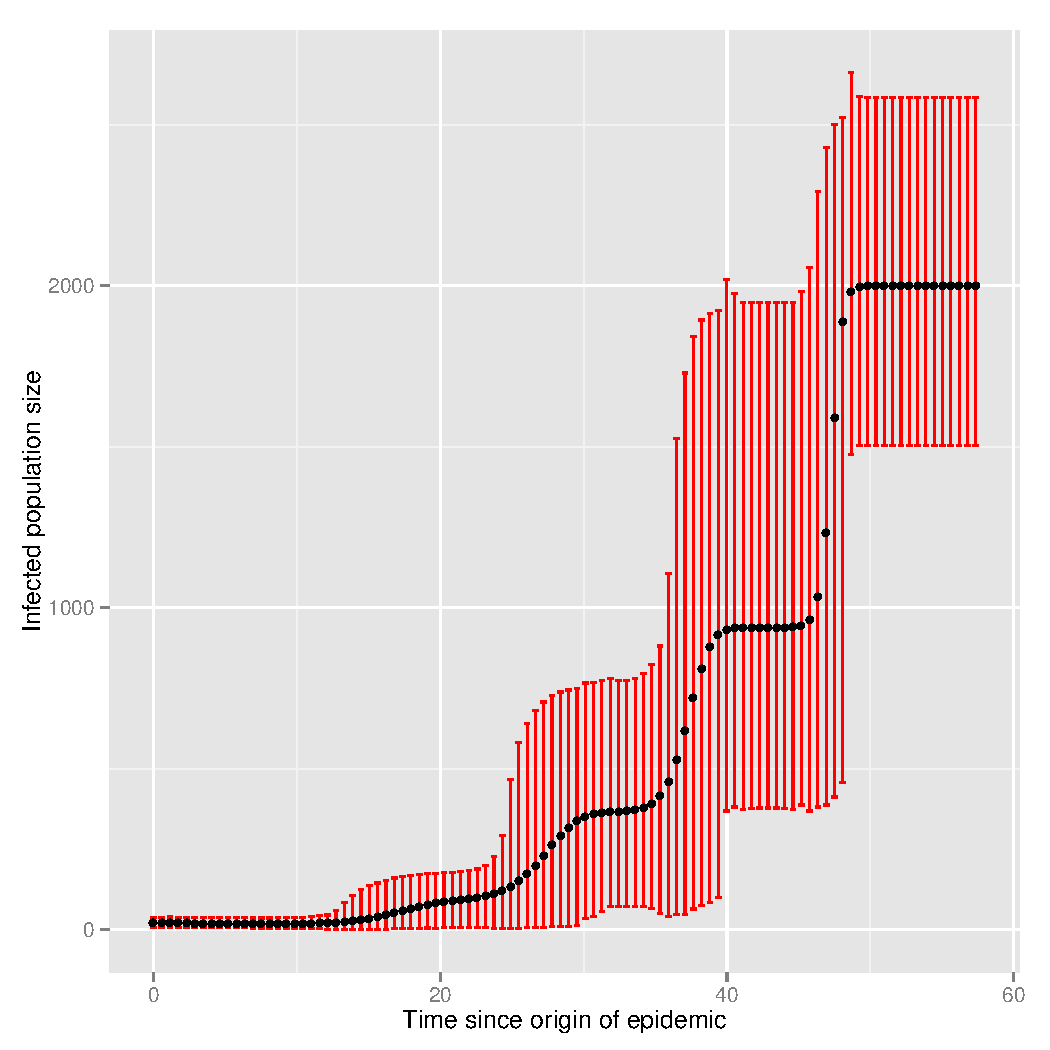
\includegraphics[width=3in]{popSize}
\caption{\footnotesize {\bf The means and 95 \% HPD intervals for posterior estimates of the infected population size through time.} 
The graph shows how the infected population size  grows through time for scG sample 1 epidemic 3 (the most recent sample from epidemic~3).} 
\label{fig: popSize} 
\end{figure}
\end{center} 

Due to the time frame we cannot yet present the results from the analysis with the birth-death skyline model with sampled ancestors. We anticipate to estimate parameters: 
\vskip2mm

\begin{tabular} {cp{0.9\textwidth}}
$\delta$ & the total rate of becoming uninfectious due to death or sampling. It can be derived as  $\mu + \psi r$; \\

$R_0$ & the effective reproductive number defined as $\frac \lambda \delta$, where $\lambda$ is a transmission rate;  \\

$s$ & the sampling proportion and can be derived as $\frac \psi {\mu + \psi}$;  and\\

$r$ & the probability that a sampled individual will not cause further infectious;
\end{tabular}

\vskip2mm

\noindent given that we know one of the parameters, $\mu$ for example.  

\section{Interpretation}

We can estimate the past epidemiological dynamics. The computation time is quite large although is feasible for datasets with approximately 300 samples. 



\section{Outlook}

To use the birth-death model, we need information about one of the parameters, such as the total rate of becoming uninfectious, i.e., the expected time from the time of infection until the time when the person stops causing other infectious due to treatment, behaviour change or death. 

\section{Supplement}

Our model allows to estimate samples that are direct ancestors of other samples in a transmission chain and removal (from epidemic) at sampling probability. Figure~\ref{fig: SA} shows preliminary posterior estimates of sampled ancestors for one of the samples. The mean estimate and 95\% HPD for $r$ was 0.9 [0.77, 0.98] for scA sample 1 epidemic 1. 
\begin{center} 
\begin{figure}[!h]
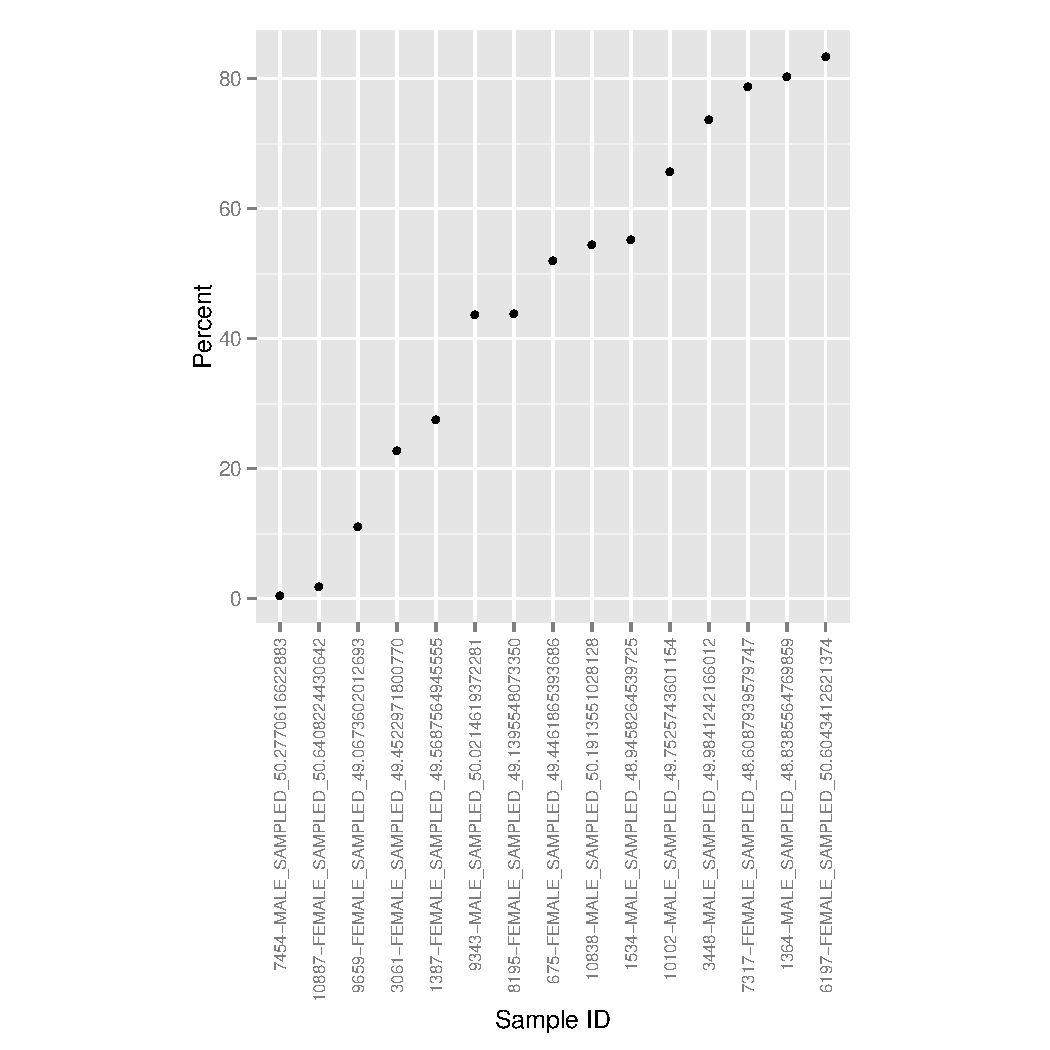
\includegraphics[width=4in]{sa_graph_scA}
\caption{\footnotesize {\bf Posterior probabilities of samples to be sampled ancestors.} 
The graph shows the posterior probabilities of samples to be sampled ancestors for scA sample 1 epidemic 1 (the most recent sample from epidemic 1). Only samples with non-zero probabilities are shown} 
\label{fig: SA} 
\end{figure}
\end{center} 

\end{document}
